%\documentclass[acmtog]{acmart}
\documentclass[acmtog, anonymous, review]{acmart}
\usepackage{subfigure}
\usepackage{algorithm2e}
\usepackage{empheq}
\newcommand*\AAnd{\textbf{ and }}
\newcommand*\AOr{\textbf{ or }}
\newcommand*\ANot{\textbf{not }}

%% \BibTeX command to typeset BibTeX logo in the docs
\AtBeginDocument{%
  \providecommand\BibTeX{{%
    Bib\TeX}}}
    
%\setcopyright{acmlicensed}
%\copyrightyear{}
%\acmYear{}
%\acmDOI{}

%\acmJournal{TOG}
%\acmVolume{}
%\acmNumber{}
%\acmArticle{}
%\acmMonth{}

\citestyle{acmauthoryear}

\begin{document}

\title[Ray Distribution Aware Heuristics for BVHs Construction in Ray Tracing]{Ray Distribution Aware Heuristics for Bounding Volume Hierarchies Construction in Ray Tracing}

\author{Lapo Falcone}
\email{lapofalcone@gmail.com}
\orcid{0009-0001-3989-3083}
\affiliation{%
  \institution{Politecnico di Milano}
  \city{Milan}
  \country{Italy}
}

\author{Marco Gribaudo}
\email{marco.gribaudo@polimi.it}
\orcid{0000-0002-1415-5287}
\affiliation{%
  \institution{Politecnico di Milano}
  \city{Milan}
  \country{Italy}
}

\renewcommand{\shortauthors}{Falcone, Gribaudo}

\begin{abstract}
  The Bounding Volume Hierarchy (BVH) is a fundamental data structure in the ray tracing algorithms to accelerate the detection of ray-scene intersections. The Surface Area Heuristic (SAH), employed during the construction of the BVH, is based on the hypothesis that the ray distribution in the scene is uniform. In this paper, we show that the SAH hypothesis is not valid when importance sampling is used, and propose two novel heuristics. With the Projected Area Heuristic (PAH) we demonstrate how it is possible to estimate better the cost of a BVH. In particular, we replace the approximation of the probability an AABB is hit by a ray, from the ratio between the surface areas of the node and the root of the BVH, to the ratio of their projected areas. The plane the AABBs are projected on and the kind of projection (either orthographic or perspective) are chosen based on the local ray distribution. With the Splitting Plane Facing Heuristic (SPFH) we show how we can build higher-quality BVHs by taking into account the knowledge of the ray distribution in a local region of the scene during the selection of the orientation of the plane used to split a node.
\end{abstract}

%% Generated by the tool at http://dl.acm.org/ccs.cfm.
\begin{CCSXML}
  <ccs2012>
     <concept>
         <concept_id>10010147.10010371.10010372.10010374</concept_id>
         <concept_desc>Computing methodologies~Ray tracing</concept_desc>
         <concept_significance>500</concept_significance>
         </concept>
   </ccs2012>
\end{CCSXML}
  
\ccsdesc[500]{Computing methodologies~Ray tracing}

\keywords{Ray tracing, Bounding volume hierarchy, Surface area heuristic, Projected area heuristic, Splitting plane facing heuristic, Monte-Carlo importance sampling}

%\received{}
%\received[revised]{}
%\received[accepted]{}

\maketitle

\section{Introduction}
The Surface Area Heuristic (SAH, \cite{sah, sah_primer}) is the cost function used in most of the state-of-the-art BVH builders. Given the root node of the BVH and a node $N$ containing $t$ triangles, the cost associated by SAH to $N$ is computed as:

\begin{equation}
  cost_{SAH}(N) = \frac{surface\;area(N)}{surface\;area(root)} \cdot t
  \label{eq:sah}
\end{equation}

The core idea behind SAH is to try to minimize the number of intersection tests that must be carried out while traversing the BVH, to find the first intersection between the ray and the scene. To achieve this result, the first term of the formula attempts to estimate the probability that a random ray hits the node $N$. Such probability is expressed as the ratio of the surface areas of the node and the root of the BVH. The Surface Area Heuristic is based on some hypotheses:

\begin{itemize}
  \item All the rays are infinitely long and never intersect a primitive of the scene;
  \item All the rays start outside the scene;
  \item All the rays hit the root of the BVH;
  \item The rays follow a random uniform distribution in the 6-dimensional\footnote{3 spatial dimensions and 3 directional dimensions.} space of the scene.
\end{itemize}

In this paper we challenge the last hypothesis of SAH, and introduce the theory of two novel heuristics that take into account non-uniform ray distributions in the scene. We then briefly present a customizable framework written in modern C++ where to test the proposed heuristics, and, eventually, show some metrics on their performance and accuracy. The C++ framework and its documentation can be found in the supplemental material.

\section{Related Work}
Papers related to the design of heuristics where one of the four SAH hypotheses is not considered valid have been quite numerous in the past, as well as articles concerned with the interaction between the Surface Area Heuristic and other techniques often used in ray tracers.

In 2015 Gu, He and Blelloch in \cite{contractions} proposed a method to modify the topological structure of a given BVH to make it more suited to be traversed by the rays belonging to the distribution present in the scene. In order to do so, they cast a small amount of rays to collect information about the intersections between them and the nodes of the BVH, and then decide whether a node should be further subdivided or merged with its sibling. Our approach is different, inasmuch we attempt to leverage the presence of local ray distributions in the scene to directly build the BVH.

The approach adopted by Gu et al. takes inspiration from \cite{bittner_havran}, where Bittner and Havran use the information gathered from the traversal of the scene via a Representing Ray Distribution (RRD) to propose an enhancement to the SAH.

In \cite{srdh} Feltman, Lee and Fatahalian propose a heuristic, called Shadow Ray Distribution Heuristic (SRDH) taking into account frequent occluders of shadow rays to build higher-quality BVHs.

The last SAH hypothesis is not the only one of interest to researchers. For instance, Fabianowski, Fowler and Dingliana with \cite{interior_rays} propose a method where the second hypothesis is considered not valid.

Hunt and Mark, with \cite{mailboxing}, propose a correction to the SAH to take into account the interaction between the SAH and the mailboxing technique often used by BVH builders.

Another work \cite{perspective_planes} from Hunt and Mark proposes to split an AABB with planes parallel to a perspective grid, instead of the cartesian planes. The goal of this method is to use a splitting plane that is parallel to the rays in a particular region of the scene, which is a similar objective to the one of our SPFH, even though reached by using a different approach.

In 2013 Alia, Karras and Laine with \cite{overlapping_heuristic} proposed the End-Point Overlapping heuristic (EPO), to show the negative impact of the overlapping between the AABBs of sibling nodes on the BVH traversal performance.

\section{SAH Last Hypothesis Falls}
In the majority of the algorithms of the ray tracing family, Monte-Carlo integration \cite{monte_carlo} is used to estimate the reflective term of the Kajiya rendering equation \cite{kajiya}:

\begin{equation}
  \int_\Omega BRDF(\bar{p}, \bar{\omega}_i, \bar{\omega}_o) \cdot \cos(\bar{n}, \bar{\omega}_i) \cdot L_i(\bar{p}, \bar{\omega}_i) d\bar{\omega}_i
  \label{eq:kajiya_reflective}
\end{equation}

In other words, the Monte-Carlo method is used to approximate the amount of light incoming ($L_i$) to the point $\bar{p}$ from all the directions belonging to the hemisphere $\Omega$, oriented toward the normal $\bar{n}$ of the surface where $\bar{p}$ lies. For each direction, the incoming light is weighted with the BRDF of the material of the surface, and with the cosine geometry term.

In order to compute how much light is coming to $\bar{p}$ from a given direction $\bar{\omega_i}$, ray tracing algorithms cast probe rays toward the $-\bar{\omega_i}$ direction. If the probe ray hits a light source, it is immediately known how much light it carries; if it hits an object, new probe rays are recursively cast to evaluate the Kajiya rendering equation at the new intersection point, and with outgoing direction $\bar{\omega_i}$.

In order to estimate the incoming light accurately, many probe rays must be cast. Indeed, the error of the Monte-Carlo estimator decreases with the square root of the number of cast rays. For instance, in order to reduce the error by a factor $2$, then $2^2=4$ times more probe rays must be traced.

An inefficiency in using plain Monte-Carlo is that, by casting the rays in random uniform directions, many of them will not contribute much to the computation of the incoming light. This can happen because a probe ray is cast toward a dark region of the scene, or because the BRDF for that specific ray direction\footnote{And for that specific outgoing direction $\bar{\omega_o}$} returns a weight close to zero.

Importance sampling can be used to reduce Monte-Carlo error without increasing the number of probe rays \cite{importance_sampling}. With importance sampling, probe rays are cast by following a Probability Density Function (PDF) proportional to the integrand, instead of uniform. In the ray tracing context the integrand is unknown, but it can be approximated. A common approach, called BRDF sampling, consists of approximating it with the BRDF function. Another relevant method is to cast probe rays in such a way that it is more likely for them to be oriented toward light sources \cite{light_sampling}.

However, if it is more likely that the rays are cast toward light sources, it follows that the ray distribution in the scene is not uniform.

\section{Influence Areas} \label{sec:influence_areas}
In particular, in the proximity to point lights, rays tend to converge to the point in space where the light source is located. This creates a pencil of lines (a radial pattern of rays), as it can be observed in figure \ref{fig:ray_distributions} (b), which we call \textit{point influence area} in the context of this paper. In the proximity of planar area light sources, rays tend to form a parallel pattern, which we call \textit{plane influence area}.

\begin{figure}
  \subfigure[Parallel rays]{\includegraphics[width=0.1\textwidth]{Images/plane_light_rays.png}}
  \quad
  \subfigure[Radial rays]{\includegraphics[width=0.165\textwidth]{Images/point_light_rays.png}}
  \caption{Ray distributions in the proximity of light sources.}
  \label{fig:ray_distributions} 
  \Description[The ray distributions]{On the left, rays are all parallel. On the right, rays all originates from one point.}
\end{figure}

In the next sections we propose two novel heuristics that are aware of the presence of influence areas in the scene, and leverage their presence to deliver estimates that more closely model what happens in a real-world scenario.

\section{Projected Area Heuristic (PAH)} \label{sec:pah}
With the Projected Area Heuristic we propose an amendment to the formula of the Surface Area Heuristic (equation \ref{eq:sah}), in particular to the part concerning the estimation of the node $N$ hit probability:

\begin{equation}
  cost_{PAH}(N) = \frac{projected\;area(N)}{projected\;area(root)} \cdot t
  \label{eq:pah}
\end{equation}

Instead of considering the ratio of the surface areas of $N$ and the root node, we use the ratio of their projected areas. The area of the AABB of the node can be projected by employing two different projection types, based on the influence area the node is \textit{immersed} into:

\begin{description}
  \item[Plane influence area] In case the node to compute the cost of is placed in a region of the scene where a distribution of parallel rays is present, it is possible to project its AABB to a plane perpendicular to the direction of the rays, by applying an orthographic projection;
  \item[Point influence area] If the AABB of the node is immersed in a region with a radial ray distribution, it can be projected by computing the perspective projection matrix generated by the pencil of rays.
\end{description}

In figure \ref{fig:aabbs_in_ray_distr} it is possible to visualize, through a simplified 2-dimensional example, why the projected area of an AABB can be a better proxy for the probability a ray hits it. The two AABBs have the same surface area, therefore, assuming they enclose the same amount of primitives, they are attributed the same cost by SAH. However, as it can be observed, the AABB at the top of the figure is hit by more rays than the bottom one. If we apply the Projected Area Heuristic, and compute the measure of the orthographic projection of both the AABBs on the plane parallel to the rays, the cost associated with each one of the two will better reflect what happens in the concrete real-world scenario.

\begin{figure}
  \centering
  \includegraphics[width=0.35\textwidth]{Images/rays_parallel_hit_prob.png}
  \caption{Two 2D AABBs immersed in a parallel ray distribution.}
  \label{fig:aabbs_in_ray_distr} 
  \Description[2 2D AABBs with the same area immersed in a parallel ray distribution]{The AABBs have the same shape, where one side is way longer than the other one. However, one is horizontal, and one is vertical. The vertical one is hit by many more rays of the distribution.}
\end{figure}

\section{Top-Level Structure} \label{sec:top_level}
Unlike the example of figure \ref{fig:aabbs_in_ray_distr}, in a real-world scene, with many light sources, different ray distributions organically arise in different regions of the scene. It is also likely that, in some areas, no relevant ray distribution is present. This scenario is different from the one where the Surface Area Heuristic operates. Indeed, the space where the SAH works is homogeneous, in the sense that the heuristic can be computed with the same algorithm and with the same parameters for any AABB present in the scene. The Projected Area Heuristic, instead, must be computed in a different way based on the location of the AABB. Furthermore, if no influence area covers a region of the scene, PAH cannot be applied to nodes overlapping that region.

For this reason, if for BVHs built with SAH having a top-level (TLAS) and many bottom-level (BLAS) structures, as described in \cite{tlas_blas}, is a performance optimization, when using PAH it becomes mandatory.

We decided to delimit the region of a plane influence area with an Oriented Bounding Box (OBB), and the region of a point influence area with a frustum, as shown in figure \ref{fig:influence_areas}.

\begin{figure}[H]
  \subfigure[Plane influence area]{\includegraphics[width=0.15\textwidth]{Images/obb_3d.png}}
  \quad
  \subfigure[Point influence area]{\includegraphics[width=0.125\textwidth]{Images/frustum_3d.png}}
  \caption{Enclosures of different influence areas}
  \label{fig:influence_areas} 
  \Description[One OBB and One frustum]{The Oriented Bounding Box is on the left.}
\end{figure}

Each influence area has an associated local BVH, which is built only with the subset of primitives that have at least one point inside the corresponding influence area. This implies that a primitive may end up being included in more than a local BVH, or none. Eventually, a global BVH is built with an algorithm favouring speed over quality, since, in principle, local BVHs should carry out most of the workload.

During the traversal phase, better detailed in section \ref{ssec:top_lvl_traversal}, a ray first attempts to traverse a local BVH it is \textit{affine}\footnote{The definition of \textit{affinity} is given in section \ref{ssec:top_lvl_traversal}} to. If an intersection with a primitive is found, it is guaranteed to be the closest one. Otherwise, the global BVH must be traversed.

It is important to note that it is guaranteed that the closest intersection is always found in the local BVH, only because we adopted a conservative approach while deciding which set of primitives is part of an influence area. Indeed, as stated above, a primitive is included in a certain local BVH if it has \textit{at least one point inside the corresponding influence area}. If, for instance, we opted to consider a primitive part of a BVH based on the position of its barycenter alone, there would have been cases where the closest hit could be missed, as can be observed in figure \ref{fig:double_area}.

\begin{figure}[H]
  \centering
  \includegraphics[width=0.32\textwidth]{Images/double_area.png}
  \caption{If a non-conservative approach is adopted while deciding which primitives are included in a local BVH, some intersections may be missed.}
  \label{fig:double_area} 
  \Description[Two influence areas (rectangles) and two triangles inside them; some rays start from one of the two.]{One triangle is fully contained in both influence areas. The other one is fully contained in the first one, but the second one only contains one point, but not its barycenter. One ray passes through the second triangle and hits the first one. This happens because this first ray represents the non conservative case (see text). The second ray hits the second triangle, and represents the conservative and correct approach.}
\end{figure}

\subsection{Top-Level Structure Traversal} \label{ssec:top_lvl_traversal}
During the traversal of the BVH, it is first necessary to detect what influence areas are \textit{affine} to the currently traced ray. With the proposition \textit{ray affine to influence area} we require both of these two conditions to be satisfied:
\begin{itemize}
  \item The ray origin is located inside the enclosing volume of the influence area;
  \item The ray direction is parallel, up to a tolerance, to the rays of the ray distribution.
\end{itemize}

The second condition, while intuitive to verify for plane influence areas, where all the rays have the same direction, is not so simple for point influence areas. In this case, indeed, the direction a ray must have for it to be parallel to the rays of the distribution, depends on the position of the ray origin. In order to find out if the ray direction is affine, it is possible to connect the origin of the ray to the focal point\footnote{The only point where the left, right, top and bottom planes of the frustum all intersect.} $O$ of the frustum, and verify if this line is parallel to the ray, up to a tolerance (figure \ref{fig:direction_affinity}).

\begin{figure}
  \centering
  \includegraphics[width=0.185\textwidth]{Images/direction_affinity.png}
  \caption{Visualization of the second affinity condition for point influence areas. Purple ray is affine, while blue one is not.}
  \label{fig:direction_affinity} 
  \Description[A frustum (trapezoid) contains two rays]{The first ray is parallel to the line connecting its origin to the focal point of the frustum. The second one is not.}
\end{figure}

For what concerns the first affinity condition, it can be checked in two ways. The most immediate one is to perform a point-OBB or point-frustum internal test for all the influence areas present in the scene. While simple to implement, this method does not scale if the number of influence areas increases. The second method is to use a spatial acceleration structure built on the influence areas. In our implementation, we opted to use an octree, whose foundations are explained in \cite{octree}.

\subsubsection{Octree Construction}
The information stored in the leaves of the octree is the influence areas present in the region of the scene the leaf encloses. By using an octree we approximate the influence areas by subdividing them into parallelepiped regions, conceptually similar to voxels. Therefore, the octree construction algorithm stops further subdividing a node when the 3D region it encloses is homogeneous with reference to the influence areas it contains, or when an arbitrary maximum level is set. In our tests we use 4 or 5 level octrees. Some visual examples can be observed in figure \ref{fig:octree_detect_leaf}, in some cases the Separating Axis Test (SAT, \cite{sat}) must be employed, which is expensive.

\begin{figure}[H]
  \subfigure[Leaf]{\includegraphics[width=0.22\textwidth]{Images/leaf.png}}
  \quad
  \subfigure[Non-leaf]{\includegraphics[width=0.22\textwidth]{Images/non_leaf.png}}
  \caption{Some potential cases the octree builder must handle to detect whether a node is a leaf or not.}
  \label{fig:octree_detect_leaf} 
  \Description[An AABB is overlapped by rectangles representing influence areas]{On the left, the first AABB is fully contained in the 2 influence areas; the second one is not even touched by any influence area. On the right, the first AABB is fully containing an influence area; another AABB has only one vertes of the influence area inside; the last AABB has not vertices of the influence area inside, nonetheless the influence area is intersecting it (imagine two A4 sheets placed one on the other one, with their centre points overlapping, but the first one is vertical and the second one horizontal).}
\end{figure}

More details on the implementation of the octree can be found in the code provided in the supplemental material.

\section{Splitting Plane Facing Heuristic (SPFH)} \label{sec:spfh}
The second novel heuristic we propose in this paper can be adopted during the phase of the BVH construction where an orientation to cut a node into its two children has to be chosen. A common technique is to choose the axis orientation in a round-robin fashion. Another often adopted method in state-of-the-art BVH builders, as mentioned in \cite{bvh_survey} and \cite{lsph}, is to split a node into its two children by a plane perpendicular to the longest dimension of its AABB. In this paper, we refer to this heuristic to choose the best splitting direction as Longest Splitting Plane Heuristic (LSPH).

Based on the paper \cite{overlapping_heuristic} from Alia, Karras and Laine, we propose the Splitting Plane Facing Heuristic (SPFH), whose objective is to reduce the overlapping between the projections of siblings nodes of a BVH, by leveraging the knowledge of the influence areas present in the scene.

One of the observations in the paper from Alia, Karras and Laine states that the overlapping between nodes in a BVH is a factor that degrades its traversal performance. The reason behind this is that, if a ray intersects both the children of a given node, then both branches of the BVH must be traversed, in fact negating the advantages of disposing of a hierarchical structure.

In the scenario laid out in this paper so far, we work with the projections of the AABBs of the nodes of the BVH, therefore we are interested in minimizing the overlapping area of the projections of the sibling AABBs.

To achieve this result, the SPFH makes it more likely to choose a splitting plane whose orientation is \textit{the least perpendicular} to the rays present in the influence area where the currently split node is immersed. Indeed, assuming the primitives are uniformly distributed inside the AABB of the node, if it is cut with a plane perpendicular to the rays present in that region of the scene, the projections of the two children will end up covering most of the area of the projection of the father, therefore generating a large overlapping area between them.

If, instead, the cutting plane is \textit{more parallel} to the rays, the overlapping projected area between the children will be reduced.


Another way to look at this is to think that, in case the cutting plane is perpendicular to the rays, the projections of the children will intrinsically tend to overlap, because the nodes are one in front of the other, with reference to the rays' direction (figure \ref{fig:ray_facing_simplest_case}). Instead, if the cutting plane is parallel to the rays, the children can only overlap because the primitives they are enclosing are not point-like entities, but have an extension. If we reduced the primitives to points, the overlapping would be null.

\begin{figure}[H]
  \centering
  \includegraphics[width=0.2\textwidth]{Images/overlapping_by_extension.png}
  \caption{The AABBs overlap because the triangles have an extension, not because they are one in front of the other.}
  \label{fig:overlapping_by_extension}
  \Description[2 triangles enclosed in 2 AABBs]{The 2 AABBs overlap due to the fact that the triangles overlap in the direction parallel to the plane normal.}
\end{figure}

\begin{figure}
  \centering
  \subfigure[$x$ axis plane]{\includegraphics[scale=0.065]{Images/x_axis_plane.png}}
  \subfigure[$y$ axis plane]{\includegraphics[scale=0.065]{Images/y_axis_plane.png}}
  \subfigure[$z$ axis plane]{\includegraphics[scale=0.065]{Images/z_axis_plane.png}}
  \caption{Visual illustration of the possible splitting plane orientations and how a ray can hit the children's AABBs. In the $z$ axis case, the AABBs are one in front of the other with reference to the ray direction, therefore they produce overlapping projections.}
  \label{fig:ray_facing_simplest_case}
  \Description[3 subfigures, each one has 2 AABBs separated by a plane]{In all the subfigures there is a ray parallel to the z axis. In the first figure the separating plane is parallel to the cartesian yz plane, therefore the ray can never intersect both the AABBs. Same in the second one, where the separating plane is parallel to the xz cartesian plane. In the last one the separating plane is parallel to the xy cartesian plane, therefore the ray hits both the AABBs.}
\end{figure}

In order to quantify the concept of \textit{how much perpendicular a plane is to a direction vector}, we employed these functions, where $\bar{v}$ is the direction of a ray in the influence area:

\begin{align*}
	value\;of\;x\;axis &= \frac{|v_x|}{|v_x|+|v_y|+|v_z|} \\
	value\;of\;y\;axis &= \frac{|v_y|}{|v_x|+|v_y|+|v_z|} \\
	value\;of\;z\;axis &= \frac{|v_z|}{|v_x|+|v_y|+|v_z|}
\end{align*}

First of all, only axis-aligned planes are considered. This shortcut is taken by the majority of the BVH builders, such as \cite{embree}, since, cutting an Axis-Aligned Bounding Box with a non-axis-aligned plane would not be efficient. Then, for each cartesian axis, it is computed how much $\bar{v}$ is facing it compared to the other axes. The values returned by these functions can be seen as how much, in percentage, $\bar{v}$ is facing each cartesian axis.

It is now possible to use these values to find out which axis-aligned plane is less perpendicular to $\bar{v}$. Let us call a plane whose normal is parallel to the axis $k$ the \textit{k-axis plane}. If the $value\;of\;k\;axis$ is large, then it means $\bar{v}$ is \textit{more perpendicular} to the k-axis plane.

Each time our local BVH builder has to choose the orientation of the splitting plane, it computes these three values. Then, based on some customizable thresholds which will be explained in section \ref{sec:implementation}, it decides whether it is worth it to cut the node with a plane with normal parallel to the axis whose value is the smallest one, or if it is better to fall back to using the LSPH.

\section{Implementation} \label{sec:implementation}
The source code of the implementation of our heuristics can be found in the supplemental material, as a link to an online repository. We used this implementation to carry out the tests whose results are presented in section \ref{sec:exp_results}. In this section, we will only briefly touch on the most relevant points of the BVH builder, while not mentioning the BVH analyzer and the octree builder, which are implemented with standard techniques and are less relevant in the context of this paper.

In our implementation, we developed a framework in modern C++, where a customizable BVH builder and a BVH analyzer are present. The main goals of our implementation can be summarized in these key points:

\begin{description}
  \item[Control over speed] We haven't aimed at writing the fastest possible BVH builder, by introducing all the state-of-the-art optimizations, or writing a GPU implementation. Our goal is to use it to carry out a theoretical comparison between our heuristics and the state-of-the-art ones, in their base environment.
  \item[Customizable] We wanted future researchers to be able to use our framework to test different possible variations of our heuristics in a simple way. For this reason, it is possible not only to customize some parameters controlling the building of the BVH, but also to inject custom functions to run in certain phases of the BVH construction, or during the analysis of the BVH and the top-level structure. In the supplemental material it is also possible to look at the documentation of the framework.  
\end{description}

\subsection{BVH Builder}
The algorithm driving the building of the BVH is summarized in the algorithm \ref{alg:build_bvh}

\begin{algorithm*}
  \caption{Summarized BVH construction algorithm.}
  \label{alg:build_bvh}
  \DontPrintSemicolon
  \SetKwFunction{FBuildBvh}{BuildBvh}
  \SetKwProg{FnBuildBvh}{BuildBvh}{:}{}
  \FnBuildBvh{\FBuildBvh{fatherNode}}{
        leftNode $\leftarrow$ [ ]\;
        rightNode $\leftarrow$ [ ]\;
        cost $\leftarrow \infty$\;
        splittingOrientations $\leftarrow$ SortSplittingOrientations(fatherNode)\;
        \ForAll{splittingOrientation : splittingOrientation}{
          childrenQuality $leftarrow$ EvaluateSplittingOrientation(splittingOrientation, leftNode, rightNode)\;
          \uIf{childrenQuality = SATISFACTORY}{
            \textbf{break}\;
          }
          \uElseIf{childrenQuality = STANDARD}{
            splittingPlanePositions $\leftarrow$ ComputeBinnedSplittingPlanesPositions(fatherNode, splittingOrientation)\;
            \ForAll{splittingPlanePosition : splittingPlanePositions}{
              [leftTmp, rightTmp] $\leftarrow$ SplitPrimitives(triangles, splittingPlanePosition)\;
              costTmp $\leftarrow$ ComputeCost(leftTmp, rightTmp)\;
              \If{costTmp < cost}{
                leftNode $\leftarrow$ leftTmp\;
                rightNode $\leftarrow$ rightTmp\;
                cost $\leftarrow$ costTmp\;
              }
            }
          }
          \uElseIf{childrenQuality = FALLBACK}{
              \textit{use fallback heuristics to find the best split}\;
          }
        }
        \If{\ANot StopCriterion(cost, leftNode, rightNode)}{
          BuildBvh(leftNode.triangles)\;
          BuildBvh(rightNode.triangles)\;
        }
  }
\end{algorithm*}

In the next sections the most relevant procedures of the algorithm will be analyzed.

\subsubsection{BVH Builder Parameters}
The behaviour of the BVH builder is controlled by a set of customizable parameters, as well as a set of customizable functions. The most relevant parameters are described in this list:

\begin{description} 
	\item[\texttt{maxLeafCost}] If a node has a cost less than this threshold, it is not further divided and becomes a leaf.
	\item[\texttt{maxLeafArea}] If a node has an area (either projected or surface depending on the cost strategy used) less than this threshold, it becomes a leaf.
	\item[\texttt{maxLeafHitProbability}] If the hit probability of this node is less than this threshold, it becomes a leaf.
	\item[\texttt{maxTrianglesPerLeaf}] If a node has fewer triangles than this threshold, it becomes a leaf.
	\item[\texttt{maxLevels}] Maximum level of the BVH.
	\item[\texttt{bins}] Once a splitting plane orientation is chosen, in our builder we adopt a binned approach to decide how to split a node into two children. This value controls how many splits to attempt. A higher value generates more accurate BVHs, but it is also more expensive.
	\item[\texttt{maxNonFallbackLevels}] If a node is located at a level higher than this threshold, the specified fallback strategies (usually SAH and LSPH) will be used to split it, instead of the default ones (usually PAH and SPFH). This threshold can be used to avoid using an expensive strategy even at deep levels, where there is less performance to gain.
	\item[\texttt{splitPlaneQualityThreshold}] $[0, 1]$
	\item[\texttt{acceptableChildrenFatherHitProbabilityRatio}]
	\item[\texttt{excellentChildrenFatherHitProbabilityRatio}] These parameters are described in the next sections.
\end{description}

\subsubsection{SortSplittingOrientations}
The customizable function \\\texttt{SortSplittingOrientations} must assign to each one of the three possible splitting plane orientations a quality value, and sort them based on this value. In our case, it implements the Splitting Plane Facing Heuristic, which is presented in section \ref{sec:spfh} of this paper, however the strategy to adopt is fully customizable.

\subsubsection{EvaluateSplittingOrientation} \label{ssec:eval_split_orientation}
The function \\\texttt{EvaluateSplittingOrientation} is responsible for deciding whether it is worth it to attempt to split the node with planes orthogonal to the provided splitting orientation. In order to take this decision, \texttt{EvaluateSplittingOrientation} takes into account the quality of the orientation computed by \texttt{SortSplittingOrientations}, the cost of the best children nodes found so far, and the custom parameters \texttt{splitPlaneQualityThreshold}, \\\texttt{acceptableChildrenFatherHitProbabilityRatio} and \\\texttt{excellentChildrenFatherHitProbabilityRatio}.

The algorithm computes the quality of the best children found up until this point. The quality is computed as the ratio of the hit probabilities of the children's AABBs and the father's AABB. The hit probability is determined by the adopted cost function, in our case it is the Projected Area Heuristic.

\begin{equation}
  children\;quality = \frac{HitProbability_{left} + HitProbability_{right}}{HitProbability_{father}}
\end{equation}

If the quality of the children is better than the threshold \\\texttt{excellentChildrenFatherHitProbabilityRatio}, the algorithm considers the two children as satisfactory, therefore no more splitting orientations should be attempted. Ideally, the sum of the hit probabilities of the children nodes should be lower than the one of the father node, however, this is not always the case, due to the possible overlapping between the two children.

In case, instead, the quality of the children is not excellent, then the quality of the current splitting plane orientation is evaluated. If the orientation has a quality greater than \texttt{splitPlaneQualityThreshold}, then the algorithm proceeds, and attempts to cut the father node with this new orientation.

On the contrary, if the orientation is low-quality, the algorithm inspects again the quality of the children nodes. If their quality is greater than \texttt{acceptableChildrenFatherHitProbabilityRatio}, then the children nodes are considered satisfactory, and no more splitting orientations are attempted. Last, if their quality is lower than \texttt{acceptableChildrenFatherHitProbabilityRatio}, then a fallback method is used to split the node into two children. In our case the fallback method is to employ the Longest Splitting Plane Heuristic and the Surface Area Heuristic.

The diagram shown in figure \ref{fig:evaluate_splitting_plane} further summarizes the procedure \\\texttt{EvaluateSplittingOrientation}:

\begin{figure}[H]
  \centering
  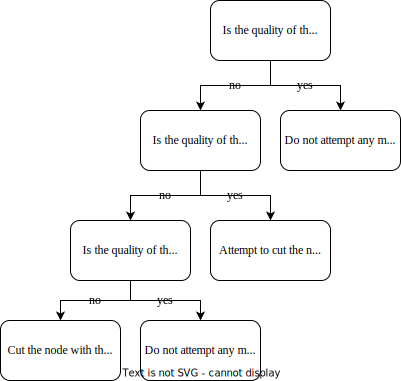
\includegraphics[width=0.45\textwidth]{Images/evaluate_splitting_plane.png}
  \caption{Decision tree of the \texttt{EvaluateSplittingOrientation} procedure.}
  \label{fig:evaluate_splitting_plane} 
  \Description[Decision tree]{The algorithm is the one described in the text.}
\end{figure}

\subsubsection{ComputeBinnedSplittingPlanesPositions}
In our builder we adopt a binned approach (figure \ref{fig:triangles_splitting_binning}) to select the position of the splitting planes by which to attempt to cut a node into its two children. After selecting the orientation, instead of trying to split a node with a plane passing through the barycenter of each primitive, we divide the length of the AABB in the chosen splitting orientation into a certain amount of regular slices. The amount of bins can be controlled with the \texttt{bins} parameter.

\begin{figure}
  \subfigure[Triangles splitting without binning]{\includegraphics[width=0.2\textwidth]{Images/split_no_binning.png}}
  \quad
  \subfigure[Triangles splitting with binning]{\includegraphics[width=0.2\textwidth]{Images/split_binning.png}}
  \caption{With binning it is possible to lose some cuts, but the most relevant ones are always found, for instance the cut dividing the blue and purple triangles.}
  \label{fig:triangles_splitting_binning}
  \Description[2 2D AABBs containing 8 triangles.]{On the left, there are several vertical lines subdividing the AABB; each line passes through the barycenter of each triangle, therefore there are 8 lines. On the right, the same exact drawing, but the lines are evenly spaced, and are only 5.}
\end{figure}

\subsubsection{SplitPrimitives}
Given the collection of primitives and a splitting plane position and orientation, generates the two children nodes. In order to decide whether a primitive is to the \textit{left} or to the \textit{right} of the splitting plane, its barycenter is considered.

\subsubsection{ComputeCost}
Given two children nodes, it computes their cost by using a customizable cost function. Along with the cost, also the hit probabilities are computed. In our case we set up the Projected Area Heuristic as the standard cost function, and the Surface Area Heuristic as fallback, but they are customizable.

\subsubsection{StopCriterion}
This customizable procedure decides whether a node is a leaf based on the \texttt{maxLeafCost}, \texttt{maxLeafArea}, \\\texttt{maxLeafHitProbability}, \texttt{maxTrianglesPerLeaf} and \texttt{maxLevels} BVH parameters.

\subsection{Influence Areas Implementation}
In our implementation we defined point and plane influence areas as implementing a general \texttt{InfluenceArea} interface. The most important methods of the interface are:

\begin{description}
  \item[\texttt{GetProjectedArea(aabb)}] returns the area projected by an AABB, based on the ray distribution associated with the concrete influence area.
  \item[\texttt{GetProjectedHull(aabb)}] returns an array of 2D points, representing the projection of the contour points of an AABB, as seen from the point of view of the influence area.
  \item[\texttt{IsDirectionAffine(ray)}] predicate deciding whether a certain ray is affine to the concrete influence area. The definition of \textit{affinity} is given in section \ref{sec:top_level}. 
\end{description}

\subsubsection{Plane Influence Area}
As described in section \ref{sec:influence_areas}, a plane influence area is described by an Oriented Bounding Box. In order to implement the \texttt{GetProjectedArea(aabb)} and \texttt{GetProjectedHull(aabb)} methods, the associated orthographic projection matrix must be computed. It can be computed starting from the eye position, which is at the centre of one of the faces of the OBB, and the extents of the OBB. An arbitrary \texttt{worldUp} direction vector must also be chosen, in our case it always points toward the positive y-axis. Given this data, the orthographic projection matrix can be computed with standard formulae.

\texttt{GetProjectedArea(aabb)} is implemented by observing that the orthographic projection of an AABB can always be split into 3 parallelograms\footnote{It can happen that some parallelogram degenerates to segments, having an area of 0.}, as shown in figure \ref{fig:parallelograms}.

\begin{figure}[H]
  \centering
  \includegraphics[width=0.1\textwidth]{Images/parallelograms.png}
  \caption{The orthographic projection of an AABB can always be split into 3 parallelograms.}
  \label{fig:parallelograms} 
  \Description[In the projection of an AABB 3 parallelograms are highlighted]{Imagine to choose a point inside a hexagon having opposite sides parallel in pairs. Imagine to choose this point so that three parallelograms create if you connect it to three points of the hexagon.}
\end{figure}

The algorithm to compute the projected area can therefore be outlined as:

\begin{enumerate}
	\item Choose any vertex of the AABB, let us call it vertex $A$.
	\item Select the adjacent vertices to $A$, called $B$, $C$ and $D$.
	\item Project the 4 vertices to the plane: \\$A' = viewProjectionMatrix \cdot A$.
	\item Compute the $\overrightarrow{A'B'}$, $\overrightarrow{A'C'}$ and $\overrightarrow{A'D'}$ vectors.
	\item Compute the areas of the three parallelograms via the cross product of the vectors corresponding to the sides: \\$Area\; parallelogram = |v \times u|$.
	\item Sum the three areas.
\end{enumerate}

For what concerns the \texttt{GetProjectedHull(aabb)} method, it is implemented by following some ideas from this paper: \cite{obb_projection}. First, we define as \textit{contour point}, any point that, after its projection, is part of the perimeter of the hull. Instead, an \textit{internal point} is a point that, after its projection, is inside the hull (figure \ref{fig:contour_internal_points}).

\begin{figure}
  \centering
  \includegraphics[width=0.3\textwidth]{Images/contour_internal_points.png}
  \caption{The projected hull of an AABB. The blue points are contour points, the purple points are internal points.}
  \label{fig:contour_internal_points} 
  \Description[An AABB is projected to a plane, the projected points are highlighted]{The projected points on the perimeter of the projected hull are blue, the internal ones are purple (see description).}
\end{figure}

In order to compute the projected hull, it is first necessary to detect what points of the AABB will be contour points after the projection, in order to avoid projecting more points (the internal points) than necessary. It can be observed that, given a plane where to project the AABB, the points making up the projected hull can be determined by simply looking at the normal direction to the plane. In particular, it is sufficient to know the sign of each component of the normal direction to detect which faces are visible.

In our implementation, a dictionary-like structure, called \texttt{hullTable}, is maintained, which, at each element, stores a list of vertices. The list of vertices stored as elements of the dictionary identifies what are the contour points of a projected AABB if it is observed from a certain direction.

In order to be able to perform a fast look-up of the \texttt{hullTable}, the structure is implemented as an array, with a particular indexing rule. The indexing rule states that each position of the array is a binary encoding of the relative position from which the AABB is looked at:

\begin{tabular}{| c | c | c | c | c | c | c |}
	\hline
	\textbf{bit} & 5 & 4 & 3 & 2 & 1 & 0 \\
	\textbf{look from} & back & front & top & bottom & right & left \\
	\hline
\end{tabular}

For example, at index $9$, which in binary is $001001$, the projected contour points in the case the AABB is seen from top and left are stored. Of course, in the $hullTable$ array there will be some empty positions, since it is impossible, for instance, to look at an AABB from top and bottom at the same time.

With the indexing of the $hullTable$ array in place, it is now possible to compute the index of the array where the contour points are stored, only based on the normal direction of the projection plane, as shown in algorithm \ref{alg:hull_table_ortho}.

\begin{algorithm}
	\caption{Given the direction of the normal to the projection plane, returns the corresponding index in the \texttt{hullTable}.}
  \label{alg:hull_table_ortho}
  \DontPrintSemicolon
  \SetKwFunction{FFindHullTableIndex}{FindHullTableIndex}
  \SetKwProg{FnFindHullTableIndex}{FindHullTableIndex}{:}{}
  \FnFindHullTableIndex{\FFindHullTableIndex{dir}}{
    i $leftarrow$ 0\;
    \textbf{if} dir.x > 0 \textbf{then} i |= 1\;
    \textbf{else if} dir.x < 0 \textbf{then} i |= 2\;
    \textbf{if} dir.y > 0 \textbf{then} i |= 4\;
    \textbf{else if} dir.y < 0 \textbf{then} i |= 8\;
    \textbf{if} dir.z > 0 \textbf{then} i |= 32\;
    \textbf{else if} dir.z < 0 \textbf{then} i |= 16\;
  }
\end{algorithm} 

\subsubsection{Point Influence Area}
A point influence area is described by a frustum, as stated in section \ref{sec:influence_areas}. Since the radial ray distribution enclosed by the frustum can be seen as generated by a pinhole camera, a perspective matrix can be associated with the point influence area. Such a matrix can be computed starting from the horizontal and vertical fields of view of the frustum, and its near and far planes.

Differently from the plane influence area case, there is no shortcut to implement the \texttt{GetProjectedArea(aabb)} method. In this case it is necessary to project the contour points and compute the area of the generated hull, by using the algorithm presented in appendix \ref{apx:hull_area_computation}.

The \texttt{GetProjectedHull(aabb)} method, is implemented by reusing a similar concept to the one used for plane influence areas. Even in this case, it is necessary to identify the contour points to avoid useless projections, and even in this case it is possible to employ the \texttt{hullTable}, but with a different indexing rule. Indeed, for a perspective projection, the relevant bit of information to detect what faces are visible, and therefore which are the contour points, is the relative position between the eye location and the AABB, instead of the viewing direction (figure \ref{fig:aabb_view_hull}).

For instance, if the AABB is seen from a point of view directly above the centre of the AABB and looking directly down, the projected hull will have as contour points the vertices of the top face of the AABB. If instead the AABB is seen from the top-left, then the contour points will be those of the top and left faces.

The indexing rule is therefore replaced by the one in algorithm \ref{alg:hull_table_perspective}.

\begin{algorithm}
	\caption{Given the eye position and the AABB, returns the corresponding index in the \texttt{hullTable}.}
  \label{alg:hull_table_perspective}
  \DontPrintSemicolon
  \SetKwFunction{FFindHullTableIndex}{FindHullTableIndex}
  \SetKwProg{FnFindHullTableIndex}{FindHullTableIndex}{:}{}
  \FnFindHullTableIndex{\FFindHullTableIndex{eye, aabb}}{
    i $leftarrow$ 0\;
		\textbf{if} eye.x < aabb.min.x \textbf{then} i |= 1\;
		\textbf{else if} eye.x > aabb.max.x \textbf{then} i |= 2\;
		\textbf{if} eye.y < aabb.min.y \textbf{then} i |= 4\;
		\textbf{else if}\; eye.y > aabb.max.y \textbf{then} i |= 8\;
		\textbf{if} eye.z < aabb.min.z \textbf{then} i |= 32\;
		\textbf{else if} eye.z > aabb.max.z \textbf{then} i |= 16\;
  }
\end{algorithm} 

\begin{figure}
  \centering
  \includegraphics[width=0.25\textwidth]{Images/aabb_view_hull.png}
  \caption{Considering the x dimension, the blue eye is inside the range of the AABB, whereas the purple one is not. The purple eye can also see the right face.}
  \label{fig:aabb_view_hull} 
  \Description[An AABB is observed by 2 points of view]{One point of view can only see the front face, because it is places in between its maximum and minimum in both the x and y axes. The other point of view can see the front and right faces, because it is placed between the maximum and minimum on the y axis, but not x and z.}
\end{figure}

Once the contour points are detected, it is possible to project them with the view-projection matrix computed beforehand.

\section{Experimental Results} \label{sec:exp_results}
As already mentioned in the section \ref{sec:implementation}, we used our implementation to perform tests on methods, with the aim of performing a comparative analysis between our heuristics and the state-of-the-art ones.

Our tests have been carried out on 8 scenes\footnote{The scene models can be found in the repository in the supplemental materials.} with different characteristics:
\begin{description}
  \item[Random100] 100 randomly created triangles in a cube region.
  \item[Random1000] 1000 randomly created triangles in the same cube region. Many overlaps.
  \item[Suzanne] The head of a low-poly monkey.
  \item[Cottage] A cottage in a simple scenery. Comprehends large primitives. 
  \item[CottageWalls] The same scene as above, but enclosed in walls. All the rays hit some geometry.
  \item[Woods] An house in a wood. Medium poly-count.
  \item[Crowd] Some detailed people enclosed in walls.
  \item[Sponza] The classic Sponza model.    
\end{description}

In each scene we artificially created an influence area, where the majority of the primitives are immersed. The influence area can be \textit{plane} or \textit{point}, and its rays can be: parallel to a cartesian axis and a cartesian plane, forming a 15° angle with a cartesian axis and parallel to a cartesian plane, forming a 45° angle with two cartesian axes and parallel to a cartesian plane, oblique (not parallel to any axis or plane).

With this setup we get to test each scene in $8$ different configurations, for a total of $64$ tests. Then, we repeated each test with all possible combinations of heuristics: PAH and SPFH, PAH and LSPH, SAH and SPFH, SAH and LSPH. The total amount of tests is therefore $256$.

The parameters to build the BVH have been found empirically, as explained in section \ref{ssec:params_tuning}, and are listed in table \ref{tab:standard_properties}.

All the numerical results can be found in the supplemental material.

\begin{table}
  \caption{The values of the parameters used to build the BVHs during the testing phase.}
	\centering
	\begin{tabular}{| l | c |}
		\hline
		\textbf{property} & \textbf{value}\\
		\hline
		\hline
		\texttt{maxLeafCost} & 0\\
		\texttt{maxLeafArea} & 0\\
		\texttt{maxLeafHitProbability} & 0\\
		\texttt{maxTrianglesPerLeaf} & 2\\
		\texttt{maxLevels} & 100\\
		\texttt{bins} & 40\\
		\texttt{maxNonFallbackLevels} & 100\\
		\texttt{splitPlaneQualityThreshold} & 0.4\\
		\texttt{acceptableChildrenFatherHitProbabilityRatio} & 1.3\\
		\texttt{excellentChildrenFatherHitProbabilityRatio} & 0.9\\
		\hline
	\end{tabular}
	\label{tab:standard_properties}
\end{table}

\subsection{PAH Accuracy}
The first analysis we performed is a comparison between the error committed by PAH and SAH while estimating the cost of a BVH. 

\begin{figure}[H]
  \centering
  \includegraphics[width=0.45\textwidth]{Images/pah_accuracy_chart.png}
  \caption{PAH versus SAH mean error chart.}
  \label{fig:pah_accuracy} 
  \Description[Line graph, percentage error on y, test cases on x]{PAH error line is always below SAH error line. PAH error is almost 0 for plane influence areas, but grows for point ones, especially oblique point case.}
\end{figure}

In order to compute the error, a method to compute the real cost of a BVH is needed. It is implemented in the traversal algorithm: each time the AABB of an internal node is hit, the cost of traversing the BVH with that ray is increased by $2$, which is the number of tests that must now be completed on the children of the node. In case a leaf is hit, the cost is increased by the number of triangles contained in the node. In this way, the SAH and PAH cost functions are mimicked, where the hit probability is taken into account by the fact that we are actually traversing the BVH.

We then computed the percentage error as:

$$
error\% = \Bigg|\frac{Real\;cost - Estimated\;cost}{Estimated\;cost}\Bigg|
$$

In the chart \ref{fig:pah_accuracy} we grouped the results by influence area. It is immediately possible to note that the Projected Area Heuristic is more accurate than the Surface Area Heuristic, in case an influence area is present in the scene. The mean error for plane influence area for PAH is $2\%$, whereas for point influence areas is $12\%$.

\subsubsection{Projected Area Culling} \label{ssec:proj_area_culling}
The projections of the AABBs to the near plane can sometimes exceed the area of the section of the near plane visible to the camera, as it can be observed in figure \ref{fig:near_plane_culling}.

\begin{figure}[H]
  \centering
  \includegraphics[width=0.3\textwidth]{Images/near_plane_culling.png}
  \caption{The 2D projected hull of the AABB is not fully contained in the viewing area of the near plane.}
  \label{fig:near_plane_culling} 
  \Description[The projected hull of an AABB exceeds the near plane area]{A section of the projection of an AABB to a plane is outside of the region of the plane delimited by the near plane area.}
\end{figure}

However, the area of the projected hull outside the near plane visible section, cannot, by definition, be intersected by any ray of the influence area. This can potentially lead to screwed estimates of the cost of the BVH. In order to avoid this, it is possible to introduce the projected area culling technique. With this technique, only the set intersection of the projected hull with the visible section of the near plane is considered. The technique is outlined in appendix \ref{apx:overlapping_hull_computation}.

\subsection{PAH and SPFH Building Performance} \label{ssec:pah_spfh}
In order to compare the PAH and the SPFH building performance to the one of the state-of-the-art heuristics, we built the respective BVHs on the exact same primitives, and compared their real traversal cost, computed as explained in the previous section. The results can be appreciated in the chart \ref{fig:pah_without_fallback_faster_chart}.

\begin{figure}[H]
	\centering
	\includegraphics[width=0.45\textwidth]{Images/pah_without_fallback_faster_chart.png}
	\caption{Cost of BVHs built with PAH and SPFH compared to ones built with SAH and LSPH.}
	\label{fig:pah_without_fallback_faster_chart}
  \Description[Line graph, BVH cost on y, test cases on x]{The PAH and SPFH line is always above the SAH and LSPH line. There is a spike of the PAH and SPFH line for the plane oblique test case. The only case where PAH and SPFH is better is the plane parallel case (70 vs 90). The point parallel and point 15 cases are close (around 80).}
\end{figure}

The results of our heuristics combined are better than the state-of-the-art ones only in the case where the plane influence area has rays parallel to a cartesian axis. Given the disappointing results, we decided to analyze each one of the two novel heuristics in isolation.

\subsection{PAH in Isolation}
The tests performed in this section follow the same methodology as the ones in section \ref{ssec:pah_spfh}, with the difference that, this time, we only adopted the Projected Area Heuristic, and paired it with the standard Longest Splitting Plane Heuristic.

\begin{figure}[H]
	\centering
	\includegraphics[width=0.45\textwidth]{Images/pah_isolation.png}
	\caption{Cost of BVHs built with PAH and LSPH compared to ones built with SAH and LSPH.}
	\label{fig:pah_isolation}
  \Description[Line graph, BVH cost on y, test cases on x]{The PAH and LSPH line is always above the SAH and LSPH line by a lot. The only case where they are at the same cost (around 90) is the plane parallel case.}
\end{figure}

The results in the chart \ref{fig:pah_isolation} show that the PAH alone, produces BVHs with a worse quality than the SAH, and also worse than using our two novel heuristics combined.

Based on the observation of the BVHs built by the PAH, we hypothesize that the reason behind this behaviour is that, in the cases where it is not possible to find a good splitting plane orientation, and therefore the children's AABBs tend to overlap regardless of the position of the splitting plane, the Projected Area Heuristic always chooses the smallest and the largest possible AABBs. This happens because the algorithm tries to minimize the cost greedily, therefore the projected area weighted by the number of triangles in each node. Since one of the two children's AABBs projections would cover almost the entirety of the father's projected area regardless, so much worth choosing the smallest possible node as its sibling, to minimize their summed cost. This does not happen with the SAH because, working with 3D AABBs, it has one more dimension where to avoid the overlapping of the siblings.

This empirical hypothesis is corroborated by the fact that BVHs built with the PAH tend to have a larger maximum level, symptom that they are not well balanced.

\subsection{SPFH in Isolation} \label{ssec:spfh_iso}
The tests performed follow the same methodology as the ones in the previous section, but this time we employ the SPFH along with the SAH for our BVHs.

In this case the results are positive, and the SPFH produces BVHs with a better quality than the LSPH, in the case their nodes are immersed in any influence area. As it is possible to observe in chart \ref{fig:spfh_isolation}, using SFPH with influence areas with oblique rays, produces BVHs of similar quality to the BVHs produced by LSPH. This is expected, since, as explained in the section about the implementation (\ref{ssec:eval_split_orientation}), SPFH falls back to using LSPH in case an acceptable split is not found, and this happens often when the rays are not parallel to any cartesian axis.

\begin{figure}[H]
	\centering
	\includegraphics[width=0.45\textwidth]{Images/spfh_isolation.png}
	\caption{Cost of BVHs built with SAH and SPFH compared to ones built with SAH and LSPH.}
	\label{fig:spfh_isolation}
  \Description[Line graph, BVH cost on y, test cases on x]{The SAH and SPFH line is always below the SAH and LSPH line, especially for parallel or 15 degrees test cases (both plane and point).}
\end{figure}

We also measured the average execution time of the computations for the SPFH, compared to the time the LSPH takes. The measurements have been carried out on our system, therefore cannot be exactly replicated. However, we are interested in the comparison between the two heuristics, rather than their absolute values. The timings are shown in the chart \ref{fig:spfh_build_time_chart}.

\begin{figure}[H]
	\centering
	\includegraphics[width=0.45\textwidth]{Images/spfh_build_time_chart.png}
	\caption{Average time spent inside the compute splitting plane function for SPFH and LSPH.}
	\label{fig:spfh_build_time_chart}
  \Description[Line chart, time in milliseconds on the y, test cases on the x]{The lines of SPFH and LSPH are very similar. On average the time is 9 milliseconds.}
\end{figure}

The time to compute SPFH and LSPH is the same. However, we measured that, by using the BVH properties presented in table \ref{tab:standard_properties}, the average amount of splitting plane orientations attempted by the SPFH is $2.1$, whereas the LSPH attempted $1.5$ different splitting plane orientations on average. The criteria to decide how many splitting plane orientations to employ are explained in section \ref{ssec:eval_split_orientation}.

\subsubsection{Siblings Overlapping}
Sibling nodes overlapping is an occurrence that lowers the quality of a BVH fast. If a ray hits a region of the scene where both the children of a node are present, both branches of the BVH must be traversed, negating the advantages brought by the hierarchical structure, as it can be observed in the chart \ref{fig:overlapping_scatter}. Our heuristic works in the 2-dimensional space where AABBs are projected, therefore we decided to analyze the overlapping of the projections of the AABBs, and evaluate whether the SPFH brings the theorized benefits.

\begin{figure}[H]
	\centering
	\includegraphics[width=0.45\textwidth]{Images/overlapping_quality_scatter.png}
	\caption{High overlapping leads to worse BVH cost.}
	\label{fig:overlapping_scatter}
  \Description[Scatter chart, BVH cost on the y, overlapping percentage at level 4 the x]{The more the overlapping percentage, the more the BVH cost. The majority of points is between the lines going from 30 percent 0 to 70 percent 250, and 50 percent 0 to 85 percent 250}.
\end{figure}

The overlapping percentage between siblings has been measured at different depths of the BVH, in particular at levels $4$, $7$, $10$, $15$ and $100$. The overlapping area can be computed with the same procedure we adopted to perform projected area culling, in section \ref{ssec:proj_area_culling}. The overlapping percentage between two AABBs having areas $A_1$ and $A_2$ can then be defined as:

$$
Node \; overlapping \; percentage = \frac{V}{min(A_1, A_2)
}$$

Where $V$ is the area of the intersection shape between the two projected AABBs.

To compute the average overlapping percentage of the whole BVH, it is possible to sum together all the overlapping areas ($V_1 + V_2 + ...$) of each pair of siblings, along with the area of the smallest of the two siblings ($A_{min1} + A_{min2} + ...$), and to compute the total overlapping percentage in the same way as presented above:

$$
Total \; overlapping \; percentage = \frac{V_1 + V_2 + ...}{A_{min1} + A_{min2} + ...}
$$

From the chart \ref{fig:pah_overlapping_children} it is possible to note how SPFH ($59\%$) is better than LSPH ($66\%$) at minimizing the overlapping. SPFH works better when rays tend to be parallel to one cartesian axis. This can be associated with two factors: 
\begin{itemize}
	\item As seen in section \ref{ssec:spfh_iso}, SPFH falls back to LSPH more often in oblique test cases;
	\item Since BVHs are made up of AABBs, if the rays are parallel to a cartesian axis, it is possible to maximize overlapping reduction, as it can be observed in figure \ref{fig:overlapping_avoidance_parallel_vs_oblique}.
\end{itemize}

\begin{figure}
  \subfigure[Parallel rays]{\includegraphics[width=0.2\textwidth]{Images/overlapping_avoidance_parallel.png}}
  \quad
  \subfigure[Oblique rays]{\includegraphics[width=0.175\textwidth]{Images/overlapping_avoidance_oblique.png}}
  \caption{Overlapping reduction works best if the rays are parallel to a cartesian axis.}
  \label{fig:overlapping_avoidance_parallel_vs_oblique}
  \Description[Projections of 2 AABBs on a plane]{On the left, the rays are parallel to a cartesian axis, and the projections of the AABBs on the plane are completely disjoint. On the right, the rays are not parallel to any cartesian axis, therefore the projections of the AABBs overlap in the centre.}
\end{figure}

We also noted that SPFH is more effective at reducing overlapping in the shallow levels of the BVH. This fact can be exploited, and it is therefore possible to use SPFH only on the higher levels of a BVH, and then directly fallback to LSPH, by tuning the \texttt{maxNonFallbackLevels} parameter.

\begin{figure}[H]
  \centering
  \includegraphics[width=0.45\textwidth]{Images/siblings_overlapping_spfh_vs_lsph.png}
  \caption{Overlapping percentage at BVH level 4.}
  \label{fig:pah_overlapping_children}
  \Description[Line chart, overlapping percentage on y, test cases on x]{SAH ans LSPH line is almost always above PAH and SPFH line, especially in parallel and 15 degrees influence areas.}
\end{figure}

\subsection{Parameters Tuning} \label{ssec:params_tuning}
\begin{table*}
  \centering
  \caption{Summary of the experiments with different BVH properties values. Underlined values are the default ones.}
  \label{tab:different_properties_summary}
    \begin{tabular}{|l|c|c|c|c|c|}
      \hline
      & \textbf{Case 0} & \textbf{Case 1} & \textbf{Case 2} & \textbf{Case 3} & \textbf{Case 4}\\ 
      \hline \hline
      \texttt{\textbf{splitPlaneQualityThreshold}} & \underline{$0.4$} & $0.1$ & $0.8$ & \underline{$0.4$} & \underline{$0.4$}\\
      \texttt{\textbf{acceptableChildrenFatherHitProbabilityRatio}} & \underline{$1.3$} & \underline{$1.3$} & \underline{$1.3$} & $1.1$ & $1.5$\\
      \texttt{\textbf{excellentChildrenFatherHitProbabilityRatio}} & \underline{$0.9$} & \underline{$0.9$} & \underline{$0.9$} & $0.7$ & $1.1$\\
      \hline
      \textbf{Average BVH cost} & $110.5$ & $88.4$ & $148.3$ & $69.1$ & $124.6$\\
      \textbf{Avg. splitting planes attempted} & $1.8$ & $2.4$ & $1.5$ & $2.0$ & $1.7$\\
      \textbf{Fallback percentage} & $0.34$ & $0.13$ & $0.68$ & $0.41$ & $0.29$\\
      \hline
    \end{tabular}
\end{table*}

In this section we will briefly analyze how, by modifying some properties during the building phase of a BVH, the resulting BVH is impacted. 

In particular, we will focus on the \texttt{splitPlaneQualityThreshold}, \\\texttt{acceptableChildrenFatherHitProbabilityRatio} and \\\texttt{excellentChildrenFatherHitProbabilityRatio} properties, and measure the BVH quality and the amount of nodes generated by using the fallback heuristics instead of the PAH and the SPFH. All the results are presented in an aggregated form, where the average value of all the executed test cases is considered. We will run the analysis on all the test cases where both PAH and SPFH are used, which are $64$ in total.

With the base values shown in table \ref{tab:standard_properties}, we obtain an average BVH quality of $110.5$. The amount of attempted splitting planes per node is $1.8$. The fallback splitting method, namely using LSPH and SAH, generates the $34\%$ of the nodes\footnote{The algorithm \ref{alg:build_bvh} explains under what conditions the fallback method is used.}.

First, we tried to lower the \texttt{splitPlaneQualityThreshold}. The result we expect from this change is to build BVHs with a better quality, at the cost of an increased build time. Indeed, with a less strict threshold on the minimum quality of a splitting plane orientation, more orientations will be attempted while trying to divide a node into its two children. The results we obtained fulfill our expectation: the average cost of the BVHs is now $88.4$, with an amount of attempted orientations per node of $2.4$. Only the $13\%$ of nodes are generated by the fallback method, because, by attempting more splitting plane orientations, it is more likely to find a good split without resorting to the SAH and the LSPH.

We then tried to raise the \texttt{splitPlaneQualityThreshold}, and obtained the opposite results. The average BVH cost increased to $148.3$, while the amount of attempted splitting plane orientations decreased to $1.5$ per node. The fallback method is used to create on the $68\%$ of the nodes.

The next set of tests we performed keeps the \\\texttt{splitPlaneQualityThreshold} constant, while modifying the \\\texttt{acceptableChildrenFatherHitProbabilityRatio} and \\\texttt{excellentChildrenFatherHitProbabilityRatio} properties.

We first tried to decrease the two properties mentioned above to values of $1.1$ and $0.7$ respectively. We expect that, with a more demanding threshold to consider a split as \textit{good enough}, the quality of the BVH will increase at the cost of having more nodes generated with the fallback heuristics. The experimental results confirm our hypotheses, as the average BVH cost decreased to $69.2$, while the fallback method is employed to create the $40\%$ of the nodes. Also, the amount of splitting plane orientations attempted increased to $2.0$ per node.

Eventually we raised \\\texttt{acceptableChildrenFatherHitProbabilityRatio} to $1.5$ and \\\texttt{excellentChildrenFatherHitProbabilityRatio} to $1.1$. Now the average cost of a BVH increased to $124.6$, the fallback heuristics generates only the $29\%$ of the nodes. The average amount of attempted splitting plane orientations per node is decreased to $1.7$.

In table \ref{tab:different_properties_summary} it is possible to look at all the results described above in a condensed form.

\subsection{Memory Footprint Theoretical Analysis}
In this section we try to estimate the memory consumption of the objects needed to support our heuristics, and compare them with the memory footprint of a standard BVH. The memory layout of each object can be observed in our implementation, provided in the supplemental material.

\subsubsection{Estimate of the Cost of a BVH}
In order to estimate the memory occupied by a BVH, it is first necessary to estimate the number of nodes in it. On average the BVHs of the test cases have $20.9$ levels, which can be approximated to $21$. A balanced binary tree with $21$ levels, has $2^{21}-1 = 2097151$ nodes, half of which are leaf nodes.

In our implementation, a node is represented by a structure holding an \texttt{Aabb}, two pointers to the children nodes and a list of triangles. We decided to keep the list of triangles in internal nodes too, for debugging and visualization reasons, even though it is only necessary for leaf nodes. For the sake of this analysis, only the leaf nodes are considered to contain a list of pointers to triangles. 

An \texttt{Aabb} is represented by a pair of 3D vectors of floating point numbers, therefore it has a weight of $4B \cdot 3 \cdot 2 = 24 Bytes$.

Assuming that floating points are stored in $4$ bytes, and pointers in $8$ bytes, an internal node has a weight of $24B + 2 \cdot 8B = 40 Bytes$. 

To compute the weight of a leaf node, the size of the array of triangles' indices array must be added. Since, in our test cases, the algorithm stopped when the number of triangles in a node was less than 3, it is possible to assume\footnote{It is also possible to have a leaf node with more than $2$ triangles, in case it was impossible to split due to the relative position of the triangles' centres.} that all the leaf nodes have $2$ triangles. In this case their weight is $40B + 2 \cdot 4B = 48B$.

We can now compute the cost of a balanced BVH with $21$ levels:
$$
(2^{21-1}-1) \cdot 40B + 2^{21-1} \cdot 48B \approx 92.27MB
$$

\subsubsection{Estimate of the Cost of an Influence Area}
When a BVH has an associated influence area, its cost must be considered. \\A \texttt{PlaneInfluenceArea} is made up of a \texttt{Plane}, a $4x4$ view projection matrix (used to accelerate the projection process), and an \texttt{AabbForObb}, which is an OBB enclosed in an AABB to be used as rejection test for intersections.

The \texttt{Plane} holds two 3D floating-point vectors, one for the passing point and one for the normal ($24 Bytes$). The \texttt{AabbForObb} contains $6$ 3D floating-point vectors, respectively for the centre, forward, right and up directions, and the half size in all directions. Furthermore, it contains an \texttt{Aabb} for the rejection tests: the total cost is $6 \cdot 3 \cdot 4B + 24B= 96 Bytes$.

The total weight of a \texttt{PlaneInfluenceArea} is:
$$
24B + 96B + 4\cdot 4 \cdot 4B = 184 Bytes
$$

A \texttt{PointInfluenceArea} is made up of a \texttt{Pov} and a \texttt{Frustum}. The \texttt{Pov} contains two 3D floating-point vectors for the viewing direction and position, and 2 floats for the $x$ and $y$ fields of view ($32 Bytes$).

The \texttt{Frustum} is a bigger structure, because it contains redundant information to improve ray-frustum collision detection. It contains a $4x4$ view-projection matrix, an array of $6$ 3D directions for the face normals, an array of $6$ 3D vectors for the edges and $8$ 3D vertices. Furthermore, it contains an \texttt{Aabb} for rejection tests. 

The total cost is:
$$
32B + 4\cdot 4 \cdot 4B + 6 \cdot 3 \cdot 4B + 6 \cdot 3 \cdot 4B + 8 \cdot 3 \cdot 4B = 336 Bytes
$$

The average cost of an influence area is therefore: 
$$
\frac{184B + 336B}{2} = 260 Bytes
$$

\subsubsection{Estimate of the Cost of an Octree}
In order to compute the size of all the structures needed for our heuristics, we first have to make some assumptions on the number of influence areas present in the scene. We will first analyze the case where just one influence area is present, and then the case where there are $20$ influence areas.

The cost of the top-level octree can be computed in a similar way to the BVH. An octree with $5$ levels is assumed, which is made up of $8^{5}-1 = 32767$ nodes, half of which are leaves.

A node of an octree holds an \texttt{Aabb}, $8$ pointers to its children and, in case it is a leaf, an array of pointers to the \texttt{Bvh}s included in the leaf. It follows that an internal node has a weight of $24B + 8 \cdot 4B = 56 Bytes$. A leaf node, assuming it contains just one BVH, has a cost of $56B + 4B = 60B$.

Therefore, the cost of the octree is: 
$$
(8^{5-1}-1) \cdot 56B + 8^{5-1} \cdot 60B \approx 1.9MB
$$

\subsubsection{Putting All Together}
In case there is only one influence area covering most of the scene, the total cost of our structures is:

\begin{subequations}
	\begin{align*}
	Total\;cost &= Cost\;local\;BVH + Cost\;influence\;area +\\ &+ Cost\;global\;BVH + Cost\;octree\\
	&= 92.27MB + 260B + 92.27MB + 1.9MB \approx 186.44MB
	\end{align*}
\end{subequations}

If we used only the global BVH, the cost would have been only $92.27MB$, which means that using our heuristics costs twice as much in terms of memory.

\noindent\rule{0.5\textwidth}{0.49pt}\\
In case there are $20$ influence areas, we assume that they contain roughly the same amount of triangles, and that only about $65\%$ of all the triangles in the scene are contained in at least one influence area. Before we assumed that the BVH has $21$ levels, is balanced and each leaf contains $2$ triangles. 

This means that the total number of triangles in the scene is $2^{21-1} \cdot 2 = 2097152$. Only $65\%$ of these are included in a BVH, therefore each BVH approximately contains $\frac{2097152\cdot0.65}{20} \approx 65000$ triangles. A balanced BVH with $65000$ triangles has a number of levels equal to\footnote{The division by $2$ comes from the fact that each leaf contains $2$ triangles on average, as we explained above.}:

$$\Big\lceil\log_2\Big(\frac{65000}{2}\Big)+1\Big\rceil = 16$$ 

A BVH with $16$ levels has a cost of:
$$
(2^{16-1}-1) \cdot 40B + 2^{16-1} \cdot 48B \approx 2.88MB
$$

It is now possible to compute the total cost of the structures needed to use our heuristics in this scenario:

\begin{subequations}
	\begin{align*}
		Total\;cost &= (Cost\;local\;BVH + Cost\;influence\;area) \cdot 20 +\\ &+ Cost\;global\;BVH + Cost\;octree\\
		&= (2.88MB + 260B) \cdot 20 + 186.44MB + 1.9MB \approx 191.22MB
	\end{align*}
\end{subequations}

Since the $20$ BVHs contain a smaller amount of nodes the cost of each BVH is greatly reduced. This relation allows us to use our structures even in cases with many influence areas of modest size.

\section{Future Developments} \label{sec:future_developments}
One important development our work would benefit from, is an improvement of the employed algorithms and data structures. While in this paper we showed the merit of PAH and SPFH from a theoretical point of view, it is now fundamental to test them in more concrete use cases, before continuing the development in other directions.

In order to do so, we suggest looking at the state-of-the-art algorithms used to build BVHs with SAH and LSPH, and adapt them to PAH and SPFH. In principle, many of the optimizations used for standard heuristics should perform equally well for our heuristics too. For instance, Stich et al. \cite{bvh_spatial_splits} idea of splitting big triangles can help SPFH in further reducing the overlapping. Tessari et al. \cite{stochastic_bvh_construction} suggest building BVHs only on a stochastically chosen subset of the primitives of the scene; despite the final BVH can be slightly lower quality, it may prove extremely useful in the building of the fallback BVH. These are just two examples of techniques that can be applied to our BVH builder, potentially with few modifications. 

A different approach is instead needed for the top-level structure. In this case it is not possible to perform a one-to-one translation from existing techniques, even though it may be worth it to study how TLAS and BLAS \cite{tlas_blas} are implemented.

Another important step would be to port the construction and traversal algorithms on parallel architectures. It may be beneficial to do this process in two steps. First, implement a concurrent builder on the CPU, by using a multi-threaded approach. This could be helpful to get insights on what are the most critical points in the change of programming model. Second, transition to a fully parallel builder on the GPU. As shown in \cite{parallel_bvh}, building a BVH is a problem that can be effectively resolved by using a parallel approach, and doing so with our heuristics should be no different, except for some considerations on the data layout to make the top-level acceleration structure as efficient as possible, especially during traversal.

In case the previous developments produce acceptable results, the next step to make our techniques operative would be to create a method to detect influence areas autonomously. At the moment, we artificially generate influence areas. While this approach could be used even in a real-world scenario, by adding influence areas where light sources are present, it could bring many improvements if it was possible to detect influence areas by providing as input the rays traced in previous frames. Thanks to this improvement, it would be possible to detect influence areas even in parts of the scene far from light sources, such as near a reflective surface like a mirror. The first method that comes to mind is clustering on the 6-dimensional space of the rays, but even other directions can be explored. In particular, it could be beneficial to try to recycle results from previous frames in order to make the influence area detection algorithms more lightweight and accurate.

Another possible development is to try a different top level structure. For example, one structure that could bring some benefits over the octree is the kd-tree \cite{kd_trees}.

\section{Use Cases and Closing Thoughts}
Bounding Volume Hierarchies are a key component of ray tracing. Their hierarchical structure is fundamental in accelerating the ray-scene intersection process, which inherently makes ray tracing faster.

Our work is too general to find specific use cases, nonetheless we can summarize the strong points of our techniques, and some possible broad application contexts.

Both the Projected Area Heuristic and the Splitting Plane Facing Heuristic work best when the rays of the influence area are parallel to a cartesian axis. Since this property is known as soon as an influence area is discovered, it is possible to decide on-the-fly whether it is worth it to use our heuristics or not. For instance, in a rendering scenario where there is a static light source, it is possible to immediately decide whether it is appropriate to generate an influence area for it. In case of a dynamic light, things can become more difficult, as it would require to decide on a per-frame basis whether it is worth it to use the BVH associated with the influence area or not. In a real-time scenario this could prove too expensive.

The Splitting Plane Facing Heuristic has proven to work well, without being more expensive to use  than the state-of-the-art LSPH, therefore it may be worth it to use it both in real-time and non-real-time scenarios. The drawback of adopting SPFH is that it can be effectively employed only in specific regions of the scene, where influence areas are present, meaning that it is necessary to build the underlying top-level acceleration structure (section \ref{sec:top_level}). This fact can hinder the use of SPFH in a real-time scenario, especially for dynamic use cases, such as dynamic lights.

Without carrying out further tests or introducing the enhancements suggested in section \ref{sec:future_developments}, we think that our heuristics are more suited for non-real-time use cases, where a faster-to-traverse BVH can reduce the rendering time even more effectively. This could change in the future.

Our work, while it has been tested on concrete scenes, is mostly a theoretical one. We showed how the novel heuristics we proposed can work in some specific scenarios. However, we think that the way to actually adopt them on concrete use cases is realistically long, but, given the potential benefits we showed they can bring, we believe it is worth it to travel it.

\bibliographystyle{ACM-Reference-Format}
\bibliography{bibliography}

\appendix

\section{Hulls Intersection Computation and Area} \label{apx:overlapping_hull_computation}
In order to find the overlapping region between two 2D hulls in 2-dimensional space, we can proceed as outlined in the diagram \ref{fig:hull_culling_algo}:

To find out what vertices of a hull are inside the other one, it is possible to loop over them and adopt the point inside convex hull test, such as the one presented in \cite{point_inside_test}.

To detect an intersection between two segments, the algorithm shown in \cite{segments_intersection} can be employed.

\begin{figure}[H]
  \centering
  \includegraphics[width=0.4\textwidth]{Images/hull_culling.png} 
  \caption{General algorithm to find the overlapping region between two convex hulls called $A$ and $B$.}
  \label{fig:hull_culling_algo}
  \Description[The algorithm]{Detect vertices of A inside B, then, detect vertices of B inside A, then detect intersection points between edges, then order vertices (if there are at least 3)}
\end{figure}

After finding the internal and intersection points of the two convex hulls, the obtained set must be ordered counterclockwise (or, arbitrarily, clockwise), so that two consecutive vertices form an edge of the convex hull.

\begin{figure}[H]
  \centering
  \subfigure{\includegraphics[width=0.21\textwidth]{Images/overlapping_hull.png}}
  \subfigure{\includegraphics[width=0.19\textwidth]{Images/vertices_sorting.png}}
  \caption{Yellow vertices are found in the first 2 steps (vertices inside), whereas light blue vertices are found in the third step (edges intersections). Vertices are then sorted counterclockwise by using the \texttt{atan2} function.}
  \label{fig:overlapping_hull}
  \Description[Visualization of the steps of the algorithm in previous figure]{On the left there are 2 overlapping convex hulls, where the points of the intersection hull are colored yellow and light blue (see caption). On the right the intersection hull has its vertices connected to its barycenter, to show their atan2 ordering.}
\end{figure}

To do so it is possible to compute the barycenter $O$ of the set of points. Given that the intersection of two convex hulls is necessarily convex, we know for certain that $O$ will be inside the convex hull formed by the vertices we found so far.

Now, for each vertex $A_k$ it is possible to calculate the vector $\overrightarrow{OA_k}$, and sort the vertices based on $atan2(\overrightarrow{OA_k}_y, \overrightarrow{OA_K}_x)$. The \texttt{atan2($v_y$, $v_x$)} function returns the angle between the positive x-axis and the vector $v=\langle v_x, v_y \rangle$. Differently from the arctangent function, the returned angle ranges in the interval $(-\pi, \pi]$, therefore it is well suited for the purpose of sorting the convex hull vertices.

\subsection{2D Hull Area Computation} \label{apx:hull_area_computation}
To calculate the area of a 2-dimensional hull, the Gauss's area formula, also known as the shoelace formula \cite{shoelace}, can be employed.

Given a polygon with vertices $P_0, P_1, ..., P_n$, where each vertex has coordinates: $P_k = (x_k, y_k)$, its area can be found with this formula:
\begin{align*}
	Area =& \frac{1}{2}\cdot\bigg|\left(\begin{vmatrix} x_0 & y_1\\y_0 & y_1 \end{vmatrix} + \begin{vmatrix} x_1 & y_2\\y_1 & y_2 \end{vmatrix} + ... + \begin{vmatrix} x_{n-1} & y_n\\y_{n-1} & y_n \end{vmatrix} + \begin{vmatrix} x_n & y_0\\y_n & y_0 \end{vmatrix}\right)\bigg|\\
	=& \frac{1}{2} \cdot \Big|\displaystyle\sum_{i=0}^{n}(x_i \cdot y_{i+1} - y_i \cdot x_{i+1})\Big| \ \ \ \ \ where \ P_0 = P_{n+1}
\end{align*}
\end{document}
\endinput
